\documentclass{standalone}
\usepackage{tikz}
\usepackage{color}
\usetikzlibrary{positioning, shapes, arrows.meta, calc, decorations.pathreplacing}

\definecolor{myblue}{RGB}{82,126,171}
\definecolor{myred}{RGB}{168, 50, 50}

\tikzset{
  square/.style={draw,outer sep=5,inner sep=3,minimum size=10,line width=0, 
    very thick, draw=myblue, top color=white,bottom color=white},
  noborder/.style={draw,outer sep=0,inner sep=0,minimum size=20,line width=1, 
    draw=none, scale=1, anchor=west},
  blue/.style={draw,outer sep=35,inner sep=3,minimum size=20, line width=1, 
    very thick, draw=none, top color=myblue, bottom color=myblue, scale=1.25}
}

\begin{document}

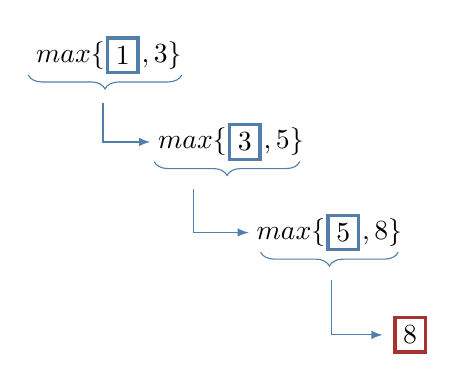
\begin{tikzpicture}[>={Latex[width=2mm,length=2mm]}]
%[1,2,5,8]
\node [square] at (-0.65,1.7) {$1$};
\node [noborder] at (-1.75,1.7) {$max\{~~~~,3\}$};
\draw[decorate,color=myblue,decoration={brace,amplitude=5pt}] (0.1,1.45) -- (-1.85,1.45);
\draw[-latex,color=myblue] (-0.9,1.1) |- (-0.3,0.6);

\node [square] at (0.9,0.6) {$3$};
\node [noborder] at (-0.2,0.6) {$max\{~~~~,5\}$};
\draw[decorate,color=myblue,decoration={brace,amplitude=5pt}] (1.6,0.35) -- (-0.25,0.35);
\draw[-latex,color=myblue] (0.25,0) |- (0.95,-0.55);

\node [square] at (2.15,-0.55) {$5$};
\node [noborder] at (1.05,-0.55) {$max\{~~~~,8\}$};
\draw[decorate,color=myblue,decoration={brace,amplitude=5pt}] (2.85,-0.8) -- (1.1,-0.8);
\draw[-latex,color=myblue] (2,-1.15) |- (2.65,-1.85);


\node [square, draw=myred] at (3,-1.85) {$8$};

\end{tikzpicture}

\end{document}
